\chapter{16 Tales - Overview}

\begin{figure}[H]
    \centering
    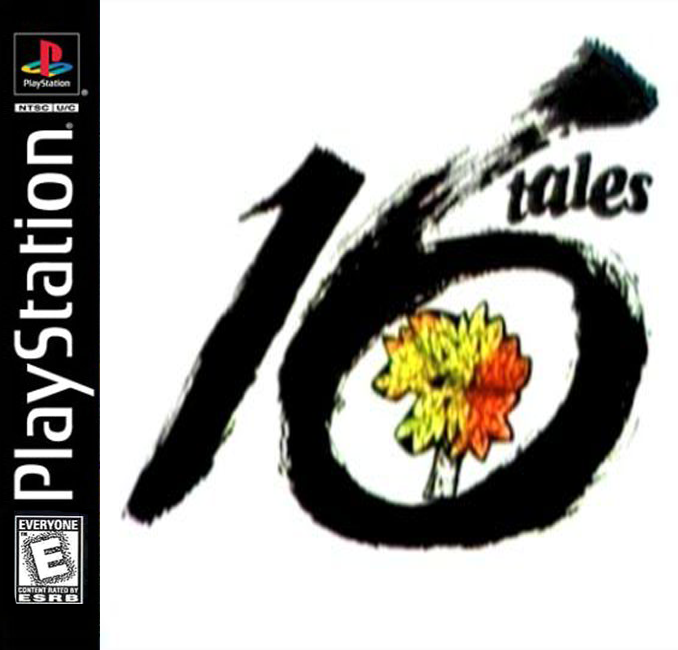
\includegraphics[width=\textwidth / 2]{"./Games/16Tales/Images/16TalesGeneralLogo.png"}
    \caption{16 Tales PlayStation 1 Logo}
\end{figure}

16 Tales is a series of eduaction video games developed by The Lightspan Partnership starting in 1996.
Each game consists of four 15-minute video programs detailing various cultures' stories and lore.

The volumes, and the cultures which are represented with the 16 Tales games are as follows:

\begin{itemize}
    \item Native American Tales
    \item East Asian Tales
    \item Spanish and Latin American Tales
    \item African Tales
\end{itemize}

To call the 4 volumes of 16 Tales video games "video games" is a bit of a misnomer.
They are more accurately described as interactive video programs, as the user has no control over the video content.
The user can only pause, rewind, and fast forward the video content, and select which video program to watch.

Through the documentation of these 4 volumes, I have attempted as accurately as possible to document the content of each of the 16 Tales video programs.
However, I cannot guarantee the accuracy of the transcripts, as for some of the content, a different language was spoken, and I occassionally had issues understanding the exact content of what was being said, as well as the spelling of some of these words.
Particularly the final 15 minute video for Volume 4, "Wakaima and the Clay Man", has some Swahili spoken, and I had difficulty understanding the exact content of what was being said.
In addition, I could not find an accurate translation of the Swahili that appeared to mean the same as the English translation that was provided directly afterwards.
In these instances, I have placed the unusual text within a pair of [square brackets] to indicate that I am unsure of the accuracy of the text.

On the website \href{https://archive.org}{archive.org}, the only 16 Tales game available to play (to use the term loosely) is Volume 2.
The other way primary that I've found that would allow me to access and play these games is through the website \href{https://vimm.net}{vimm.net}, which allows you to stream the games through a PlayStation 1 emulator.
I've actually found this website to be the most reliable method to "play" the games, as the quality of the stream on vimm.net is incredibly high quality in comparison to the stream of the game on archive.org.
This website is also the method by which I've been able to play other games produced by The Lightspan Partnership, so it was a great find.
The only way other way that I've been able to access the contents of this game is through watching YouTube videos of the game, which are few and far between.

Each of the 15 minute video programs in the 16 Tales games have an option to have an audio summary of the game provided to the user, although the summaries provided for these videos are not what I have placed as the descriptions in each of the tables for each volume.

Although many of the other games produced by The Lightspan Partnership have associated merchandise, I have not been able to find any merchandise associated with the 16 Tales games.

On a final note, the music used in the introduction and outro of each video is Sun Valley, composed by David Snell.